\section{A historical context of interference and interferometers}

    Interference is the most direct fingerprint of the wave nature of light: when two beams
    overlap, their amplitudes - not their intensities - add, and the result can be brighter
    than either beam alone or, astonishingly, complete darkness. From this simple superposition
    principle grew the interferometer, an instrument that turns the invisible phase of a light
    wave into a visible pattern of fringes, and which became one of the most precise measuring
    devices ever built.

    Although Robert Hooke and Isaac Newton both studied the coloured fringes produced by thin
    films - the phenomenon still known as Newton's rings, carefully described in Newton's
    \textit{Opticks} of 1704 \cite{newton1704opticks} - neither interpreted them as evidence
    of waves. Newton's immense authority, and his corpuscular theory, held the field for a
    century. The decisive break came in 18011804 with Thomas Young, whose double-slit
    experiment showed that light passing through two narrow apertures produces a pattern of
    bright and dark bands that can only be explained if the two beams alternately reinforce and
    cancel one another \cite{young1804bakerian}. Young introduced the very word
    ``interference'' and, with it, the principle of superposition that underlies all of wave
    optics.

    Young's qualitative insight was forged into a quantitative theory by Augustin-Jean Fresnel,
    who combined the principle of interference with Huygens's secondary wavelets to compute
    diffraction and interference patterns in full detail, and whose recognition that light is a
    transverse wave (developed with Arago) tied interference firmly to polarisation: only
    components sharing a polarisation can interfere. By the middle of the nineteenth century the
    wave theory was secure, and interference had become a tool. Hippolyte Fizeau and Léon
    Foucault used interferometric methods to compare the speed of light in different media, and
    Fizeau exploited the visibility of fringes to infer stellar properties - an idea far ahead
    of its time.

    The instrument that defines the modern era is the Michelson interferometer. Albert A.\
    Michelson, seeking ever more precise measurements, built in the 1880s a device that splits
    a beam in two, sends the halves along perpendicular arms, and recombines them so that any
    difference in optical path appears as a shift of the fringes. With it, Michelson and Edward
    Morley performed in 1887 their famous experiment to detect the motion of the Earth through
    the luminiferous aether; the null result \cite{michelson1887relative} became one of the
    experimental pillars on which Einstein's special relativity would later rest. Michelson also
    turned his interferometer into a metrological standard, measuring the length of the standard
    metre in wavelengths of light, work for which he received the Nobel Prize in 1907.

    Almost simultaneously, Charles Fabry and Alfred Perot introduced in 1899 an interferometer
    of a different kind, based on multiple reflections between two highly reflecting parallel
    surfaces \cite{fabry1899theorie}. The FabryPerot interferometer produces extremely sharp
    transmission fringes and offers very high spectral resolving power; it is the direct
    ancestor of the optical resonators and cavities that define the modes of every laser. Other
    configurations followed - the MachZehnder interferometer, with its separated paths ideal
    for probing transparent samples, and the Sagnac interferometer, sensitive to rotation and
    the heart of modern optical gyroscopes.

    The visibility of the fringes in any of these instruments is not merely an experimental
    nuisance: it is a direct measure of the coherence of the light, and it was precisely the
    analysis of fringe visibility that motivated the statistical theory of coherence developed
    in a later chapter. In the twentieth century, interferometry reached almost unimaginable
    sensitivity: the Laser Interferometer Gravitational-Wave Observatory (LIGO), a pair of
    kilometre-scale Michelson interferometers, detected in 2015 the passage of a gravitational
    wave by measuring a change in arm length thousands of times smaller than a proton
    \cite{abbott2016observation}. From Young's two slits to the detection of colliding black
    holes, the interferometer has remained the same idea - read the phase of a wave by letting
    it interfere with itself - refined to extraordinary perfection.

\section{How does interference occur?}

    Lets consider two sources of electromagnetic field, under the conditions we've mentioned on this lectueres, we're going only to focus on the electric component, therefore, lets suppose we've got the following two sources of electric field
    \begin{align}
        & \vec{E}_1\left(\vec{r},t\right) = \vec{E}_1(\vec{r})e^{-i\omega_1 t},\\
        & \vec{E}_2\left(\vec{r},t\right) = \vec{E}_2(\vec{r})e^{-i\omega_2 t},
    \end{align}
    where the complex field amplitudes are given by
    \begin{align}
        & \vec{E}_1(\vec{r}) = E_1(\vec{r})e^{i\varphi_1(\vec{r})}\hat{e}_1,\\
        & \vec{E}_2(\vec{r}) = E_2(\vec{r})e^{i\varphi_2(\vec{r})}\hat{e}_2.
    \end{align}

    Theses complex field amplitudes are almost general, here the polarization vectores $\hat{e}_1,\hat{e}_2$ are'nt space-time dependent, which, in general, is what it's observed. The phases $\varphi_1(\vec{r}), \varphi_1(\vec{r})$ represent an arbitrary wavefront behavior,also $E_1(\vec{r}),E_2(\vec{r})$ represent arbitrary amplitudes. Thus the expressions above are general experessions for arbitrary sources of radiation. 

    The interference appears in the superposition of two or more electric fields, therefore, to study the interference of these two field in a space-time point $(\vec{r},t)$ we're going to add these two as follows
    \begin{equation}
        \vec{E}(\vec{r},t) = \vec{E}_1(\vec{r},t) + \vec{E}_2(\vec{r},t).
    \end{equation}

    As we've explained before, measuring the electric field is really hardo to do, so what we study and see are the irradiencies or radiations intensity, also the frequencies $\{\omega_1,\omega_2\}$ are too fast time oscillations for the human eye and most of the detectors, so we only can study their time averages. Having all this on count, lets calculate the average of the irradiances
    \begin{align*}
        & \left\langle \left|\left|\vec{E}(\vec{r},t) \right|\right|^2\right\rangle = \left\langle \left|\left|\vec{E}_1(\vec{r},t) \right|\right|^2\right\rangle + \left\langle \left|\left|\vec{E}_2(\vec{r},t) \right|\right|^2\right\rangle + 2\left\langle Re\left\{\vec{E}_1^*(\vec{r},t)\cdot \vec{E}_2(\vec{r},t) \right\}\right\rangle,\\
        & \left\langle \left|\left|\vec{E}(\vec{r},t) \right|\right|^2\right\rangle = \left|\left|\vec{E}_1(\vec{r})\right|\right|^2 + \left|\left|\vec{E}_2(\vec{r})\right|\right|^2 + 2 Re\left\{ \vec{E}_1^*(\vec{r})\cdot\vec{E}_2(\vec{r}) \left\langle e^{-i(\omega_1-\omega_2)t} \right\rangle \right\}.
    \end{align*}

    The first two terms corresponds to \textbf{the total field intensity} and the third terms is called \textbf{the interference term}because it contains the interaction of both fields.

    From a mathematical point of view, to make the interaction non zero, both frequencies must be the same $\omega_1=\omega_2$, this, like most books say, should imply that the interference only ocurrs with two sources with the same frequency or on identical photons but, this is not completely correct. The frequency-difference exponential $\exp\left(-i \left[\omega_1 - \omega_2 \right]t\right)$ is, in general, not zero, so \textbf{there are a lot ultrafast oscillations and interferences} what we see, and what we detected using measuring instruments is the time average, and in average, these are zero.

    Before going further, lets define the field intensisties as
    \begin{align}
        & \left|\left|\vec{E}_1(\vec{r}) \right|\right|^2 = I_1(\vec{r}),\\
        & \left|\left|\vec{E}_2(\vec{r}) \right|\right|^2 = I_2(\vec{r}).
    \end{align}

    The interference terms is then given by
    \begin{equation}
        \vec{E}_1^*(\vec{r})\cdot \vec{E}_2(\vec{r}) = E_1(\vec{r})E_2(\vec{r})e^{i \left[ \phi_2(\vec{r}) - \phi_1(\vec{r})\right]}\hat{e}_1^*\cdot\hat{e}_2,
    \end{equation}
    then the field intensity is
    \begin{equation}
        I = I_1 + I_2 + 2Re\left\{\left(\hat{e}^*_1\cdot \hat{e}_2\right)e^{i\triangle\phi (\vec{r})} \right\} \underbrace{E_1(\vec{r})E_2(\vec{r})}_{\left(I_1I_2\right)^{1/2}}.
    \end{equation}

    The functional $\triangle\phi = \phi_2(\vec{r}) - \phi_1(\vec{r})$ is known as the phase-difference of the waves. The intereference term is zero if the \textbf{polarisations are orthogonal} this means $\hat{e}^*_1\cdot\hat{e}_2 = 0$. Without any loss of generality an only for mathematical convenience\footnote{In fact, the polarisation here is only an contrast modulator, however, when we study the spatial coherence, the polarisation is even more important and conditionates the behavior of the interference.} we're going to consider both sources have got the same polarisation, this means $\hat{e}_1 = \hat{e}_2 \rightarrow \hat{e}_1^* \cdot \hat{e}_1 = 1$. Thus, the total intensity becomes
    \begin{equation}\label{eq:GenInterferenceTerm}
        I = I_1 + I_2 + 2\left(I_1 I_2\right)^{1/2} \cos\triangle\phi = \left(I_1 + I_2\right)\left(1 + 2\frac{\left(I_1I_2\right)^{1/2}}{I_1+I_2}\cos\triangle\phi\right).
    \end{equation}

    The equation \ref{eq:GenInterferenceTerm} is the our most general expression for the interference. Lets notice that the intereference terms is composed in two parts: the first one is a relation between the two intensities $I_1,I_2$ and the second one only depends of the phase-difference of the two sources by a cosine, then, \textbf{the real interference becomes in the phases not in the intensities}, the first terms only \textbf{modulates the visibility} of the interference, and we then can call it $\mathcal{V}$ and write it as
    \begin{align}
        & \mathcal{V} = 2 \frac{\left(I_1 I_2\right)^{1/2}}{I_1+ I_2} = \frac{I_{max} - I_{min}}{I_{max} - I_{min}},\\
        & I_{min} = \left(I_1^{1/2} - I_2^{1/2} \right), \quad I_{max} = \left(I_1^{1/2} + I_2^{1/2} \right),
    \end{align}
    this term $\mathcal{V}$ is called the \textbf{visibility factor} which module the constrast on the interference fringes. 
    

    \subsection{Interference of plane waves}

        The expression \ref{eq:GenInterferenceTerm} is, as we said, the general interference expression, so lets apply it to two plane wave sources.  For the plane wave we've got that the complex amplitudes are given by
        \begin{equation}
            E_1(\vec{r},t)= E_1 e^{i\left(\vec{r}\cdot\vec{k} + \varphi_1\right)}, \qquad E_2(\vec{r},t)= E_2 e^{i\left(\vec{r}\cdot\vec{k} + \varphi_2\right)},
        \end{equation}
        where, we are going to suppose, just for to make the maths a bit easier but the methodology is the same, that both amplitudes are the same $E_1 = E_2$. 

        Because, we are considering that the both waves have got the same frequency $\omega_1 = omega_2$ this implies that both have the same wave number amplitude, this means $||\vec{k}_1|| = ||\vec{k}_2|| = k$. Then, we will have that the phase-difference term is given by
        \begin{equation}
            \triangle\phi = \left(\vec{k}_2 - \vec{k}_1\right)\cdot\vec{r} + \varphi_2 - \varphi_1.
        \end{equation}

        The interference \ref{eq:GenInterferenceTerm} having on count that $I_1 = I_2 = I_0$ is then
        \begin{equation}
            I = \left(I_0 + I_0\right)\left(1 + 2 \frac{\left(I_0 I_0\right)^{1/2}}{I_0 + I_0}\cos\triangle\phi\right) = 2I_0\left[1 + \cos\left(\vec{K}\cdot r + \triangle\varphi \right)\right],
        \end{equation}
        where $\vec{K} = \vec{k}_2 - \vec{k}_1$ is the interferences vector. To understand bettwer the intereference, we're going to do a bit of geometry (see figure \ref{fig:PlaneWaveInterferences}).
        
        \begin{figure}[h]
            \centering
            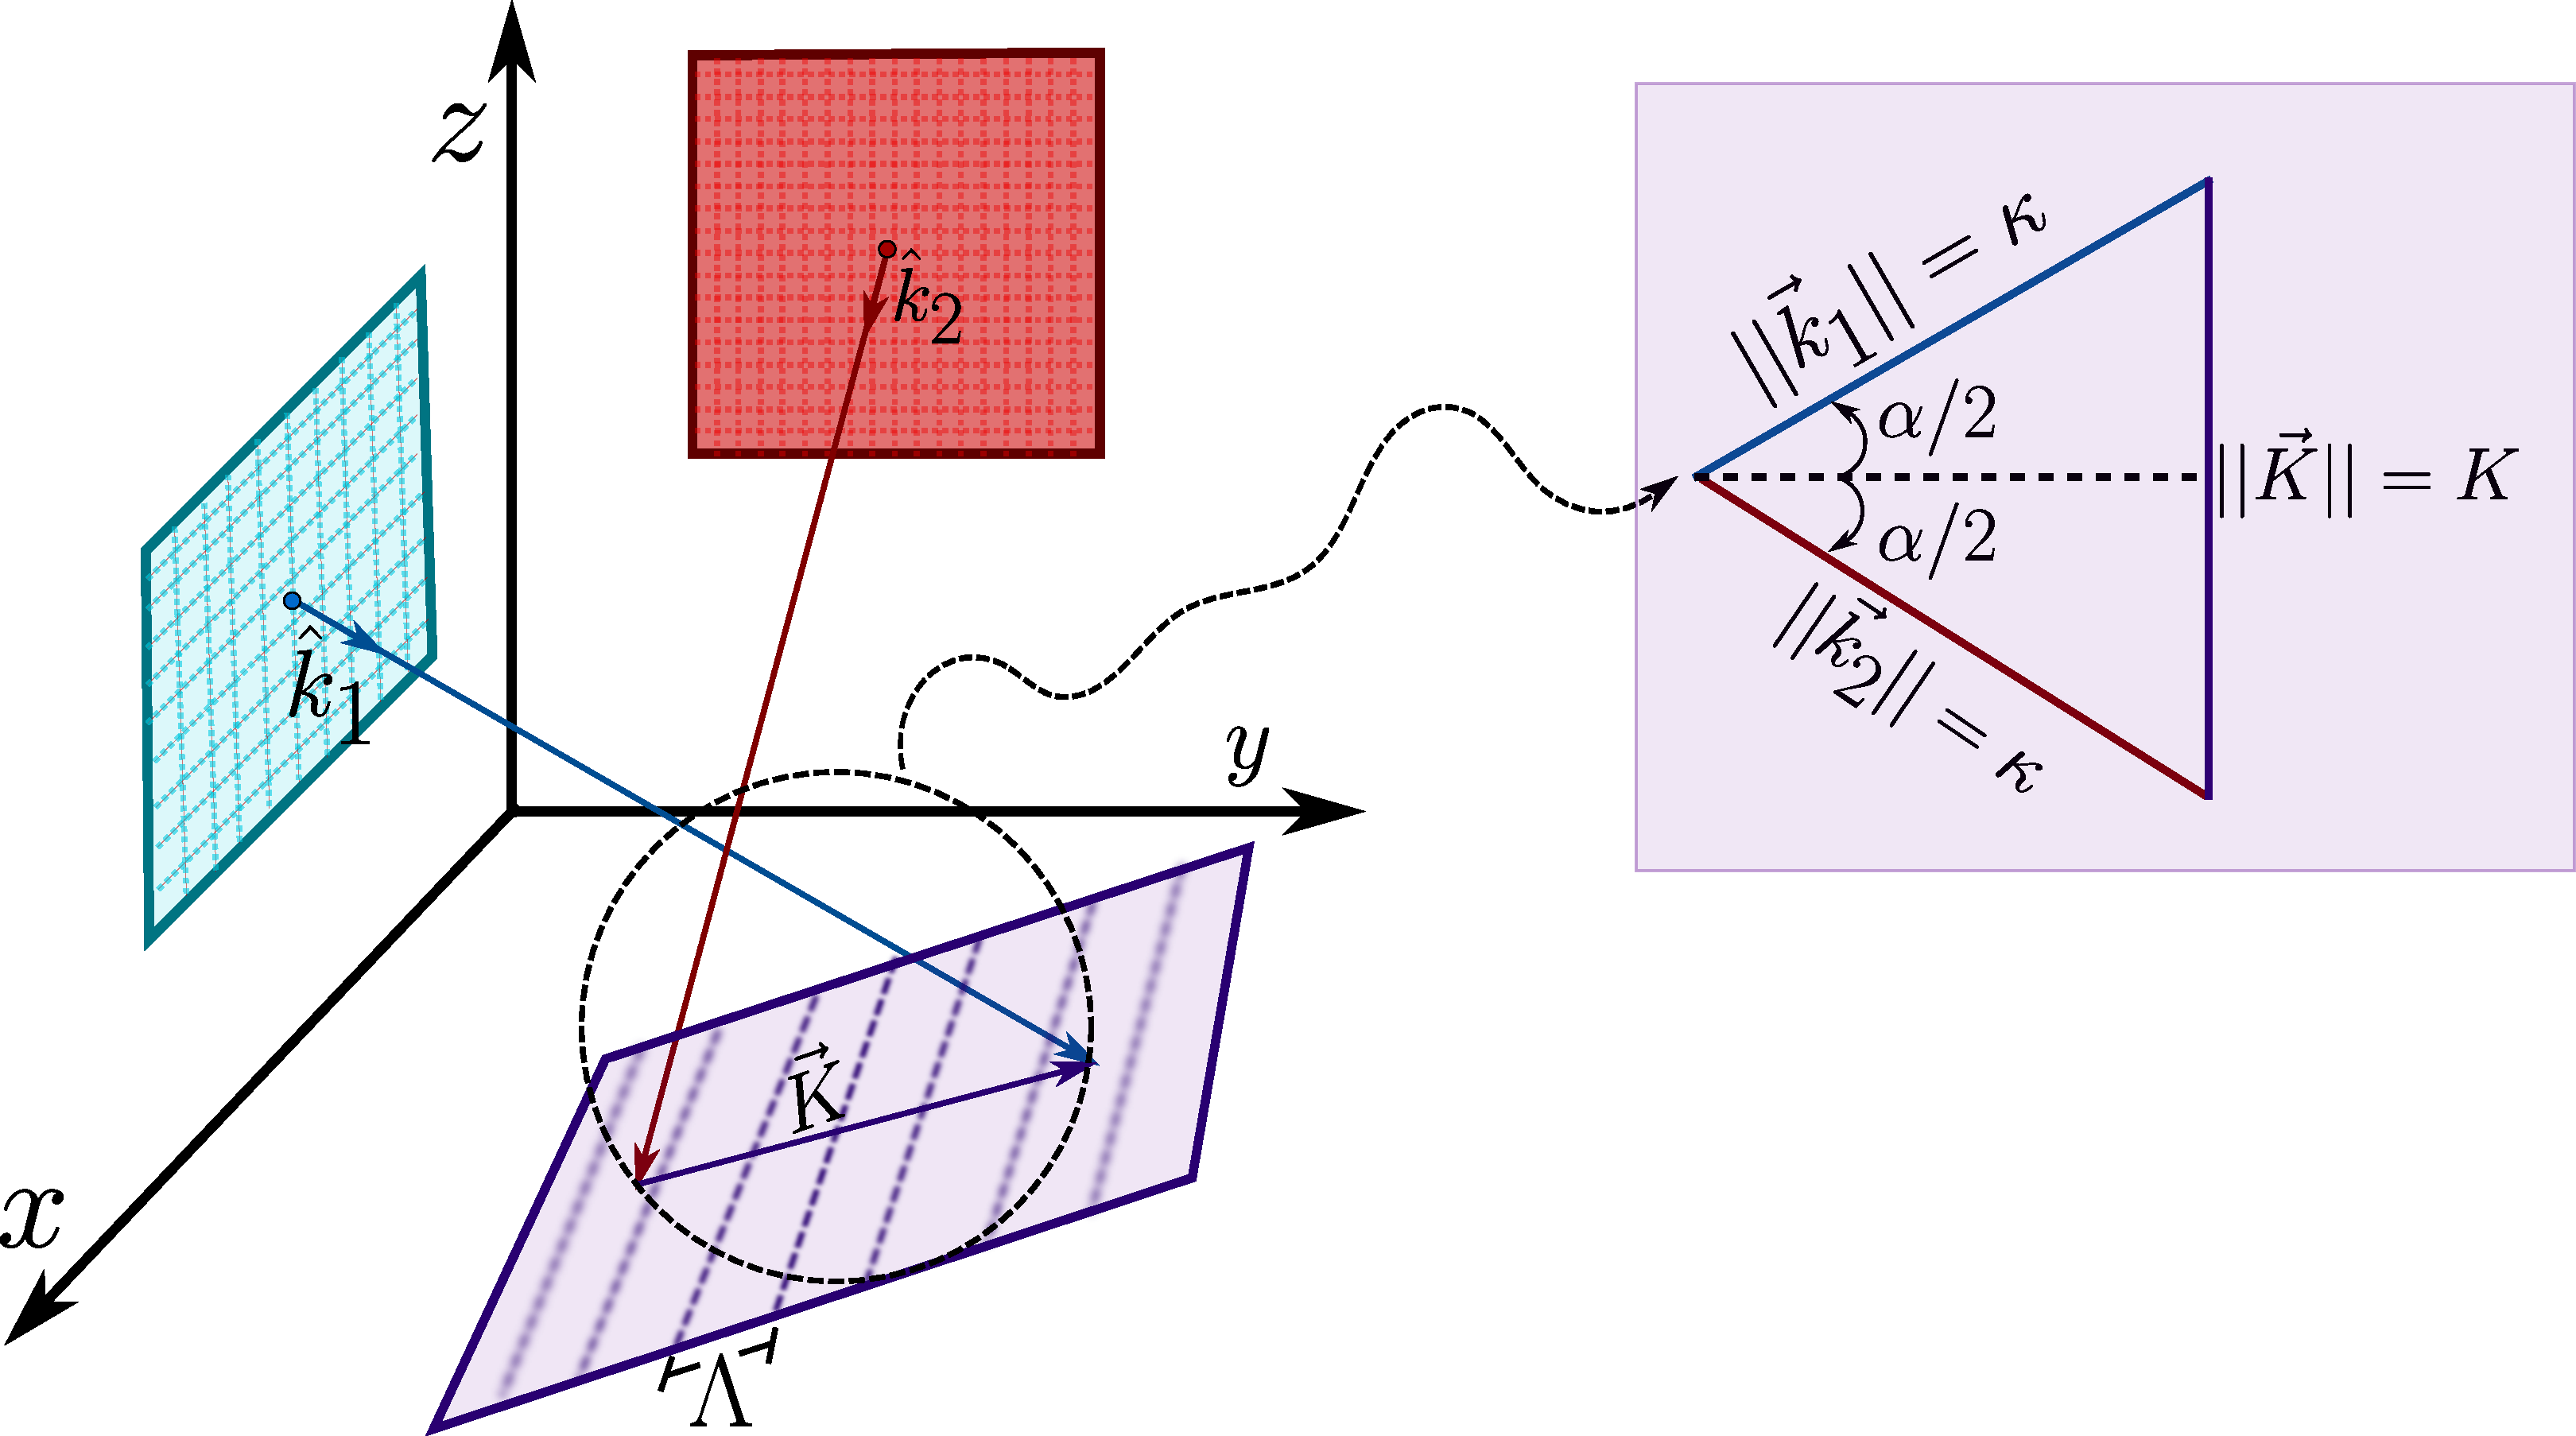
\includegraphics[width = 0.9\textwidth]{Chapter 4/Figures/PlaneWavesInterferences.pdf}
            \caption{Two plane waves with unitary number vector $\hat{k}_1,\hat{k}_2$ propagate and interferece producing a pattern of interference characterized by a vector $\vec{K}$ and an interfringe distance $\Lambda$.}
            \label{fig:PlaneWaveInterferences}
        \end{figure}

        Because we're interested on the interference plane, we will take to $\vec{r} = X\hat{x}$ on the interference plane, where $\hat{x} = \vec{K}/ ||\vec{K} ||$, then the spatial dependce gets the form

        \begin{equation}\label{eq:PlaneLambda1}
            \vec{K}\cdot \vec{r} = KX = 2\kappa X \sin\left(\frac{\alpha}{2}\right),
        \end{equation}
        and because $K$ is a wave number vector on the interference plane, it can be written in terms of its wave-lenght,which orresponds to the interfringe distance $\Lambda$ as
        \begin{equation}
            K = \frac{2\pi}{\Lambda},
        \end{equation}
        then 
        \begin{equation}\label{eq:PlaneLambda2}
            \vec{K}\cdot \vec{r} = \frac{2\pi}{\Lambda}X.
        \end{equation}

        To calculate the relation between the interfringe distance $\Lambda$ an the known parameters of the wave, we're going to equate the equations \ref{eq:PlaneLambda1} and \ref{eq:PlaneLambda2} therefore
        \begin{align}
            & \frac{2\pi}{\Lambda}X = \frac{2\pi}{\lambda}X\sin\left(\frac{\alpha}{2}\right),\\
            & \Lambda = \frac{\lambda}{2\sin\left(\frac{\alpha}{2}\right)},
        \end{align}
        where we used that $\kappa = \frac{2\pi}{\lambda}$. With this term, we finally got that the total intensity in the interference of two plane wave is given by

        \begin{equation}
            I = 2I_0 \left[1 + \cos\left(\frac{2\pi}{\Lambda}X + \phi\right)\right].
        \end{equation}

        We can see that the interfringe distance $\Lambda$ behaves in a very logique way. In $\alpha \to 0$ then $\Lambda \to \infty$ this means, when the two wave number vector $\hat{k}_1,\hat{k}_2$ gets each time more parallel, the interfringe distance tends to infinity, this means, there won't be any interference pattern. 

        In the other way, if $\alpha \to \pi/4$ then $\Lambda \to min$ this means, when the two wave number vectors tend to be $45$° separeted the interfrence distance is the minimum, being clrear for us to see the interference pattern. 

    \subsection{Interference of spherical waves}

        \begin{figure}[h]
            \centering
            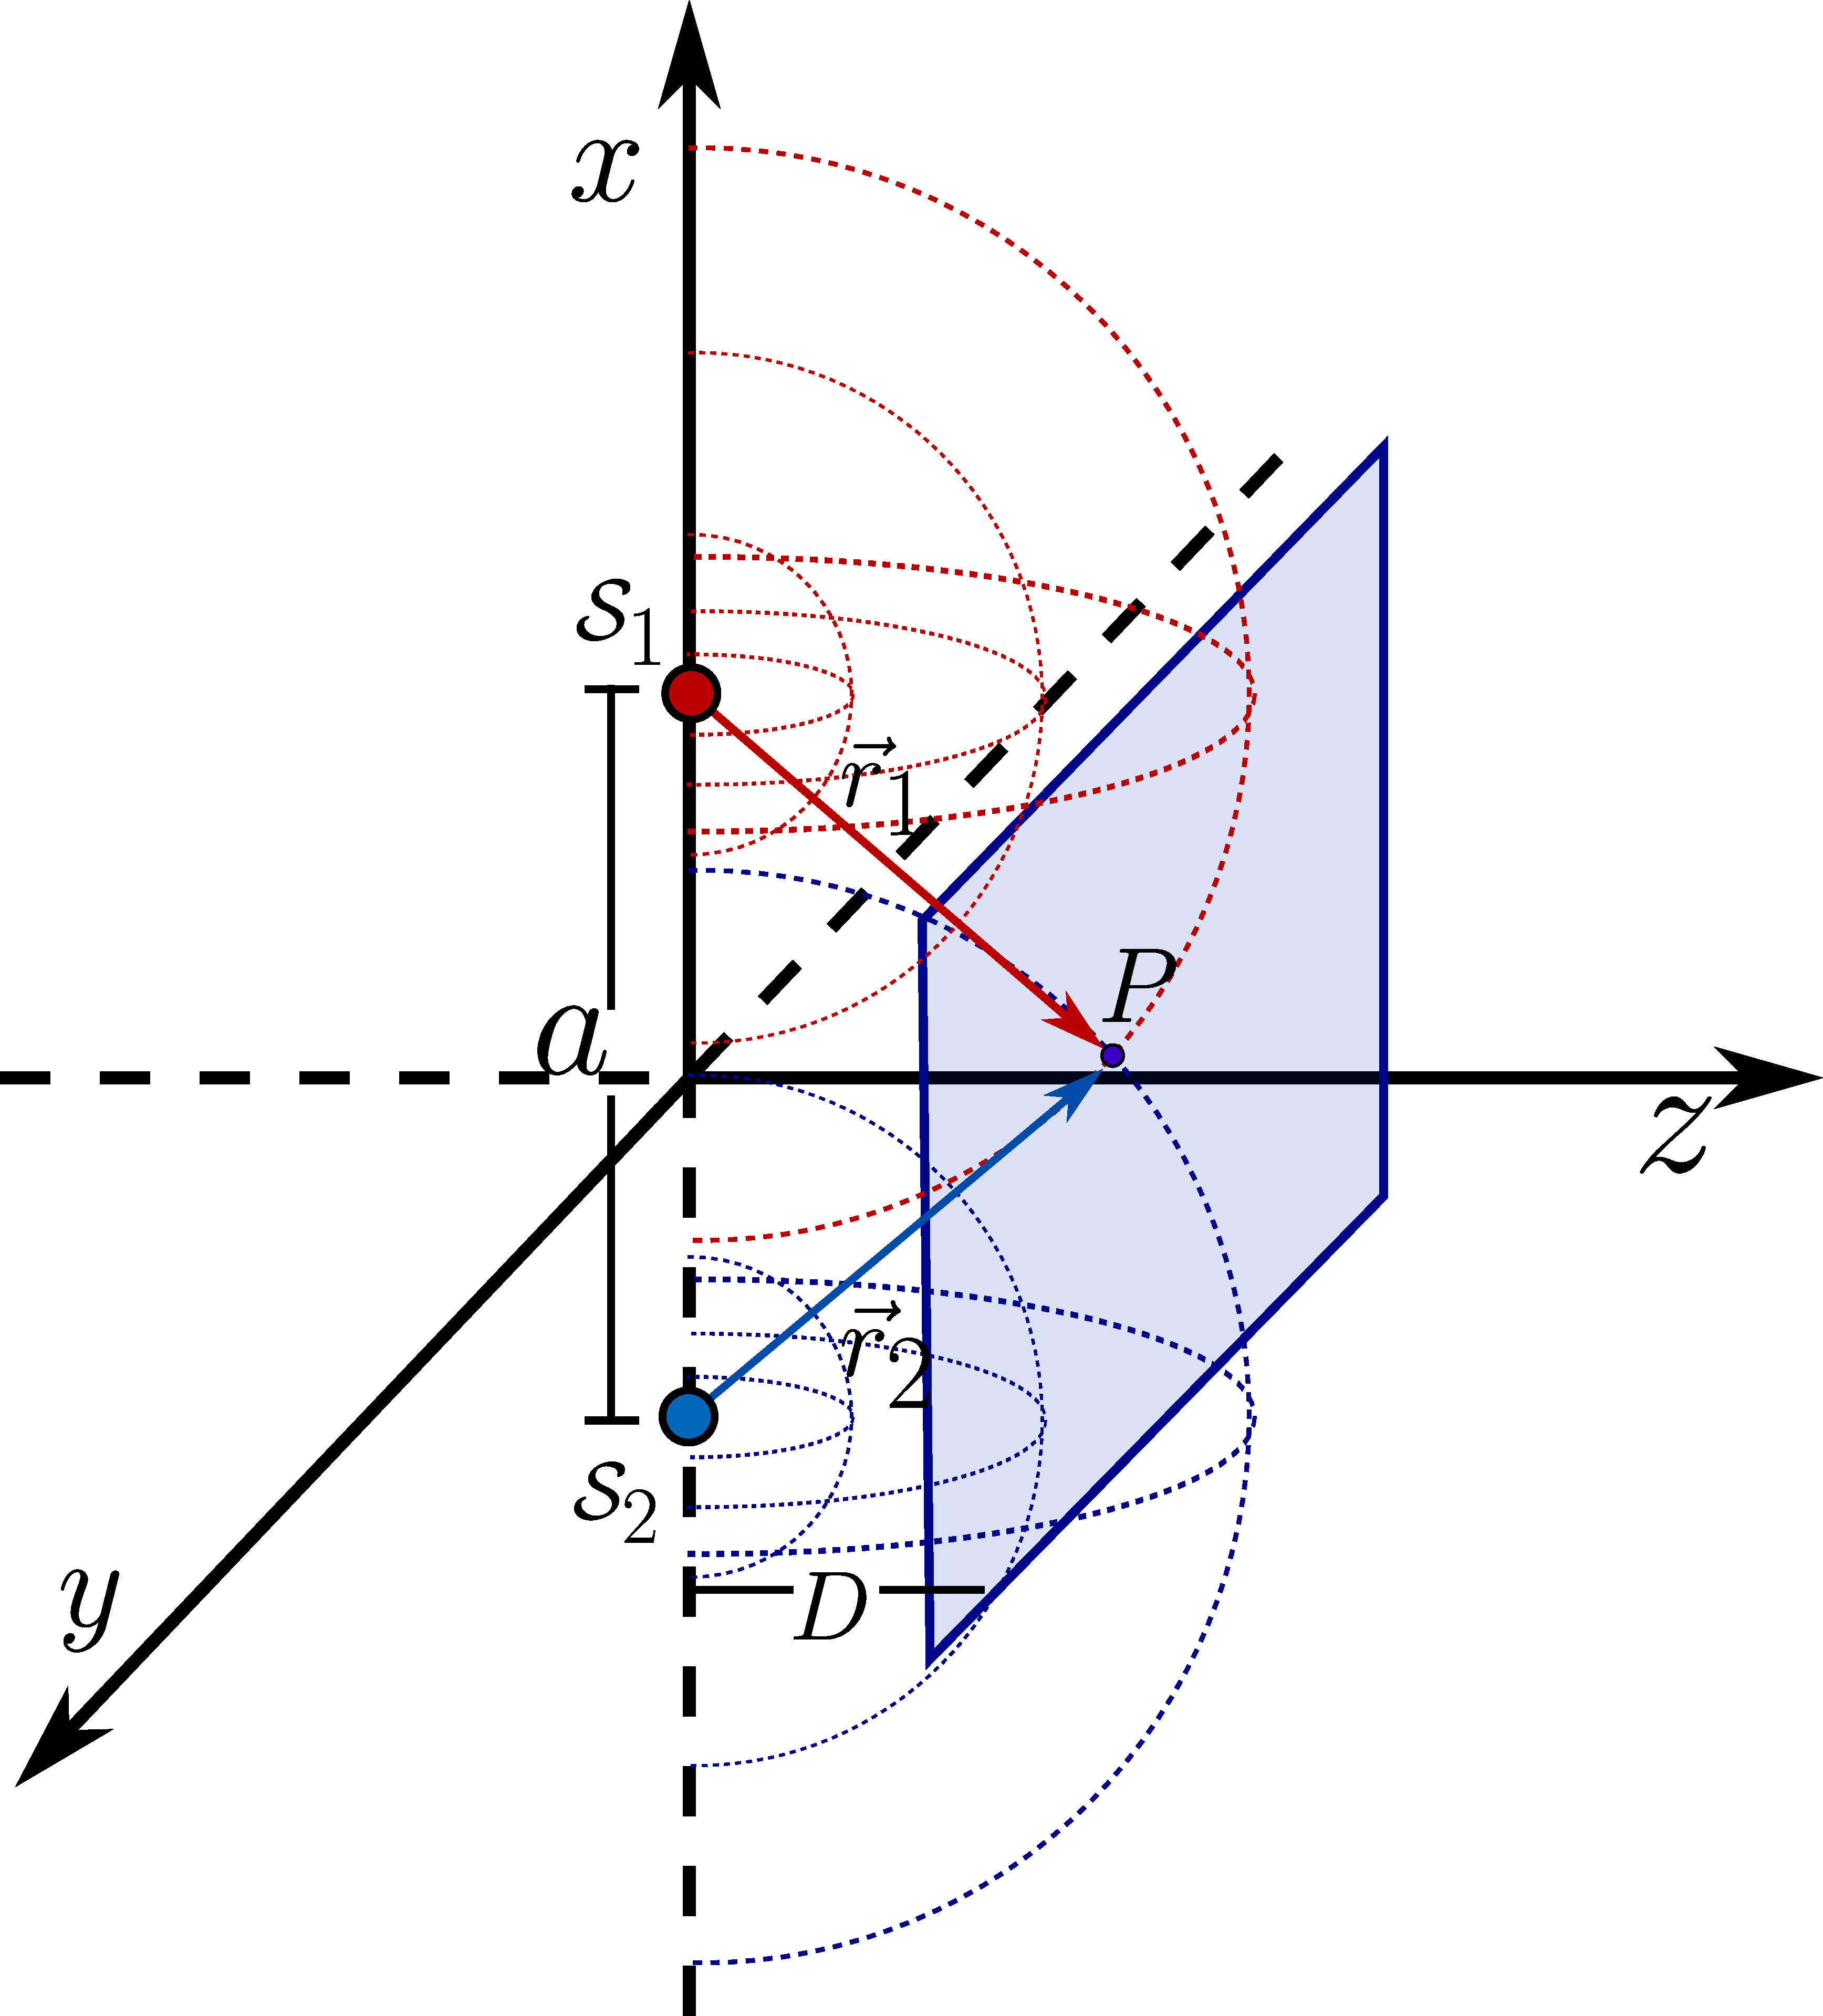
\includegraphics[width = 0.6\textwidth]{Chapter 4/Figures/SphericalWavesInterferences.pdf}
            \caption{Two plane sources of spherical waves interfere in a point $P$ located on the interference plane. The two sources are separated a distance $a$ an the distance from both surface to the interference plane is $D$.}
            \label{fig:SphericalWaveInterferences}
        \end{figure}
        
        In a similar way to the last section about plane waves, we're going to consider two radiation sources which propagte as spherical waves, so the electric field waves are given by

        \begin{align}
            & E_1(\vec{r}) = \frac{E_1}{r_1} e^{i\left(k r_1 + \varphi_1 \right)},\\
            & E_2(\vec{r}) = \frac{E_2}{r_2} e^{i\left(k r_2 + \varphi_2 \right)}.
        \end{align}
        And, again, we're going to consider, without any loss of generality just for aesthetical purposes, that both have got the sample amplitude $E_1 = E_2=E_0$. Also, lets suppose a point $P$ on the interference plane and that the two point sources are separated a distance $a\;[m]$ and both sources are separated a dsitance $D\;[m]$ as is shown in the figure \ref{fig:SphericalWaveInterferences}.

        We have got that $r_1 = \overline{\mathcal{S}_1P}$ and $r_2 = \overline{\mathcal{S}_2P}$, then the fase difference is given by
        \begin{equation}
            \triangle\phi (r) = \kappa \left(r_2-r_1\right) + \triangle \varphi.
        \end{equation}

        And we are going to consider that the field amplitudes, in a neighborhood of $P$ change very little with $r_1$ and $r_2$, and then
        \begin{equation}
            \frac{E_0}{r_1} \approx \frac{E_0}{r_2} = E,
        \end{equation}
        the intensity is then given by

        \begin{equation}
            I = 2I_0 \left\{1 + \cos\left[\kappa \left(r_2-r_1\right) + \triangle\varphi \right]\right\},
        \end{equation}
        before going further, see that the \textbf{surfaces of equal intensity $\mathbf{r_2-r_1}=cte$ are hyperboloids with focii in $\mathcal{S}_1,\mathcal{S}_2$}.

        In a plane parallel to $\overline{\mathcal{S}_1\mathcal{S}_2}$ at a distance $z=D$ two hyperbolids are produced. For $r_1 \approx r_2$ and $D \gg a$ this hiperboloids are practically planes. Therefore

        \begin{align}\label{eq:TaylorR1}
            & r_1 = \left[D^2 + \left(x - \frac{a}{2}\right)^2 + y^2\right]^{1/2} = D \left[1 + \frac{x^2}{D^2} + \frac{y^2}{D^2} + \frac{a^2}{4} - ax\right]^{1/2},
        \end{align}
        applying taylor series  to first order of $\sqrt{1+x} \approx 1 + x/2 $ we've got
        \begin{equation}
            r_1 \approx D\left[1 + \frac{x^2+y^2}{2D^2} + \frac{a^2}{2D^2} - \frac{ax}{2D^2}\right],
        \end{equation}
        and in the same way for $r_2$
        \begin{equation}\label{eq:TaylorR2}
            r_1 \approx D\left[1 + \frac{x^2+y^2}{2D^2} + \frac{a^2}{2D^2} + \frac{ax}{2D^2}\right].
        \end{equation}

        Substracting \ref{eq:TaylorR2} from \ref{eq:TaylorR1} we then we will have that the phase difference is then
        \begin{equation}
            \triangle\phi = \kappa \left(r_2-r_1\right) + \triangle\varphi \approx \frac{\kappa aX}{D} + \triangle\varphi,
        \end{equation}
        then the total intensity in the interference is given by
        \begin{equation}
            I = 2I_0 \left[1 + \cos\left(\kappa \frac{aX}{D} + \varphi_2-\varphi_1 \right)\right],
        \end{equation}
        where again 
        \begin{equation*}
            KX = \frac{\kappa aX}{D} = \frac{2\pi}{\lambda}\frac{aX}{D},
        \end{equation*}
        but $K = 2\pi/\Lambda$, being again $K$ the magnitude of the resultante wave number vector on the plane interference, and $\Lambda$ the interfringe distance. Thus the relation between $\Lambda$ an the known paramaters of both waves is 
        \begin{equation*}
            \frac{2\pi}{\Lambda} = \frac{2\pi aX}{D} \longrightarrow \Lambda = \frac{\lambda D}{a}.
        \end{equation*}

        With this result, we can see that when the two sources get closer $a \to 0$ the interfringe $\Lambda \to \infty$ this means, the interference is going to disappear when the two point sources get together.

\section{Interferometers}

    \subsection{Young interferometer}

    \subsection{Michelson and Morley interferometer}